\graphicspath{ {./hardware_installation/pictures/} }
\section{Hardwaresetup}
This section describes the setup of the hardware. It should show you,
how the boards are connected together.

In picture \ref{ESP32-CAM-USB-TO-TTL} you can see the setup of the ESP32 CAM Board connected to the USB-to-TTL module.

\begin{figure}[H]
\centering
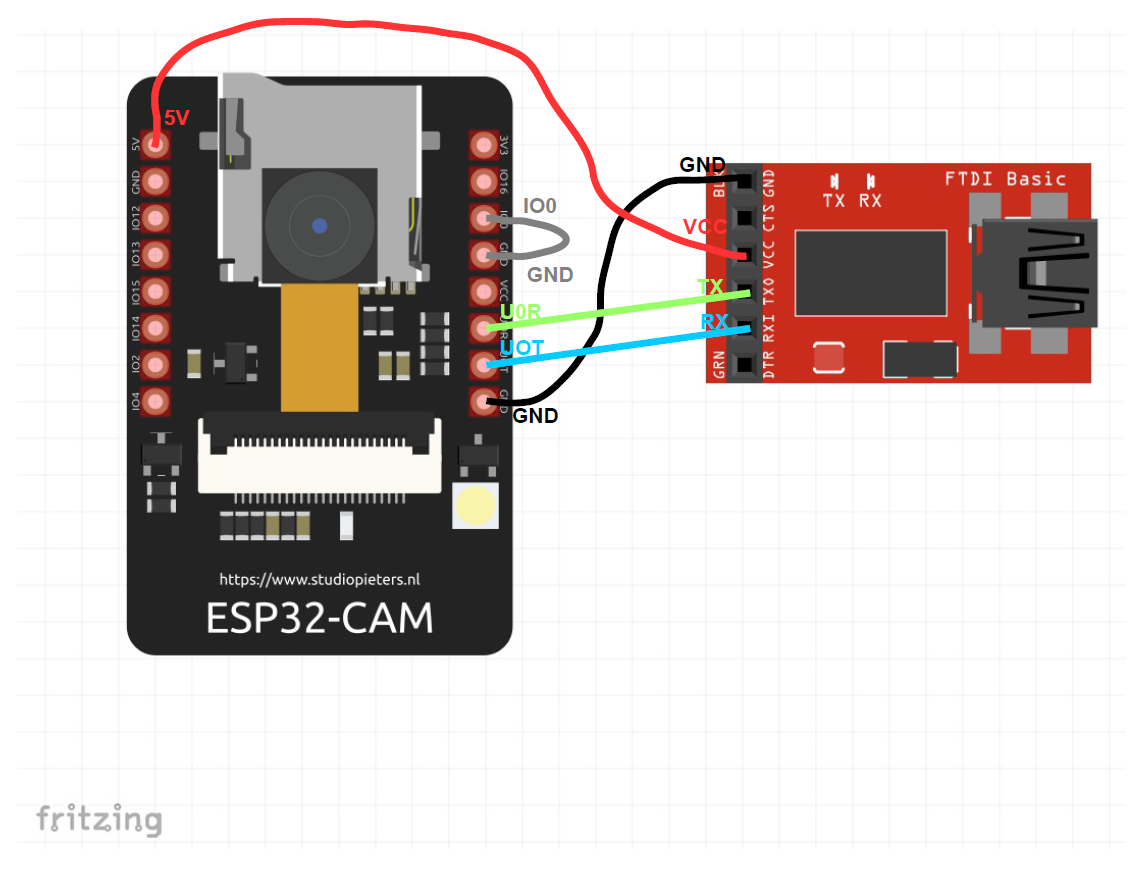
\includegraphics[width=\textwidth]{esp32_cam-ftdi}
\caption[ESP32 CAM Board connected with USB-to-TTL module]{ESP32 CAM Board connected with USB-to-TTL module \\ Origin Source: \url{https://github.com/AchimPieters/Fritzing-Custom-Parts/blob/master/Fritzing\%20Parts/ESP32-CAM_FRONT_2.png}\\ from Achim Pieters \\ License: \href{https://opensource.org/licenses/MIT}{MIT}}
\label{ESP32-CAM-USB-TO-TTL}
\end{figure}

% Please add the following required packages to your document preamble:
% \usepackage[table,xcdraw]{xcolor}
% If you use beamer only pass "xcolor=table" option, i.e. \documentclass[xcolor=table]{beamer}
\begin{table}[H]
\begin{tabular}{|l|l|l|}
\hline
Port USB-to-TTL-Module & PORT ESP32-CAM & PORT ESP32-CAM \\ \hline
GND                    & GND            & -              \\ \hline
VCC                    & 5V             & -              \\ \hline
TX                     & U0R            & -              \\ \hline
RX                     & U0T            & -              \\ \hline
-                      & GND            & IO0            \\ \hline
\end{tabular}
\caption{\label{tab:Port-Connections}Connections between the ports}
\end{table}

\fcolorbox{red}{pink}{{\fontencoding{U}\fontfamily{futs}\selectfont\char 66\relax}For the flashing mode it is needed that IO0 is connected with ground!}
